\begin{frame}[label=conclusion, standout]
    \begin{center}
    \LARGE How to approach?
    \end{center}
\end{frame}

\begin{frame}
    \begin{center}
        \Large{Break it down into smaller subproblems.}
        
        \begin{figure}
            \includegraphics[width = 0.5\textwidth]{breakcube}
        \end{figure}
    \end{center}
\end{frame}

\begin{frame}{Breaking into smaller sub-problems}
    \large Suppose we have two sequences

    \begin{center}
    
\begin{adjustbox}{max totalsize={\textwidth}{0.5\textheight}}
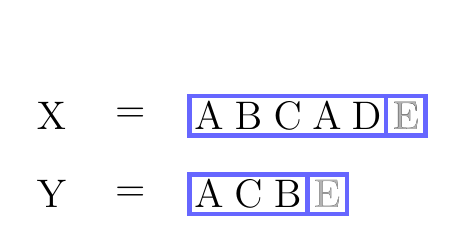
\begin{tikzpicture}

    \node at (0,3) {};
    \node at (2,2) {};

    \node[rectangle] at (-1,2) {\Large{X}};
    \node[rectangle] at (0,2) {\Large{=}};
    \node[rectangle] at (1,2) {\Large{A}};
    \node[rectangle] at (1.5,2) {\Large{B}};
    \node[rectangle] at (2,2) {\Large{C}};
    \node[rectangle] at (2.5,2) {\Large{A}};
    \node[rectangle] at (3,2) {\Large{D}};
    \onslide<1-4>{\node[rectangle] at (3.5,2) {\Large{E}};}
    \onslide<5>{\node[rectangle, text = gray!60] at (3.5,2) {\Large{E}};}
    \onslide<6->{\node[rectangle] at (3.5,2) {\Large{F}};}
    \onslide<10>{\node[rectangle, text = gray!60] at (3.5,2) {\Large{F}};}
    

    \node[rectangle] at (-1,1) {\Large{Y}};
    \node[rectangle] at (0,1) {\Large{=}};
    \node[rectangle] at (1,1) {\Large{A}};
    \node[rectangle] at (1.5,1) {\Large{C}};
    \node[rectangle] at (2,1) {\Large{B}};
    \onslide<1->{\node[rectangle] at (2.5,1) {\Large{E}};}
    \onslide<5,9>{\node[rectangle, text = gray!60] at (2.5,1) {\Large{E}};}

    
    \onslide<2,6-7>{\draw[ultra thick, blue!60] (3.5-0.25,2-0.25) rectangle (3.5+0.25,2+0.25) ;}
    \onslide<3>{\draw[ultra thick, green!80] (3.5-0.25,2-0.25) rectangle (3.5+0.25,2+0.25) ;}
    \onslide<8>{\draw[ultra thick, red!60] (3.5-0.25,2-0.25) rectangle (3.5+0.25,2+0.25) ;}

    \onslide<2,7>{\draw[ultra thick, blue!60] (2.5-0.25,1-0.25) rectangle (2.5+0.25,1+0.25) ;}
    \onslide<3>{\draw[ultra thick, green!60] (2.5-0.25,1-0.25) rectangle (2.5+0.25,1+0.25) ;}
    \onslide<8>{\draw[ultra thick, red!60] (2.5-0.25,1-0.25) rectangle (2.5+0.25,1+0.25) ;}


    \onslide<4,10>{\draw[ultra thick, blue!60] (1-0.25,2-0.25) rectangle (3+0.25,2+0.25) ;}
    \onslide<4,9>{\draw[ultra thick, blue!60] (1-0.25,1-0.25) rectangle (2+0.25,1+0.25) ;}

    \onslide<9>{\draw[ultra thick, blue!60] (1-0.25,2-0.25) rectangle (3.5+0.25,2+0.25) ;}
    \onslide<10>{\draw[ultra thick, blue!60] (1-0.25,1-0.25) rectangle (2.5+0.25,1+0.25) ;}

    

    

\end{tikzpicture}



\end{adjustbox}
\end{center}

\onslide<3->{Longest Common Subsequence : \_\_\_\_\_\_\_\_\_\_\_\_\onslide<3-5>{E}}
    
\end{frame}